\chapter{BFS}
Otra forma de recorrer el grafo es mediante el uso de la búsqueda en anchura, BFS. 

Esto lo que tiene la ventaja es que permite encontrar la distancia mínima desde el nodo inicial hacía los otros vértices. Definimos la distancia entre el nodo \(a\) y \(b\) como la menor cantidad de aristas que es necesaria cruzar para ir del vértice \(a\) al vértice \(b\).


Como imaginarás, la BFS se realiza igual que como vimos en las búsquedas, pero los estados son los vértices y las transiciones son las aristas de cada nodo. 

\begin{minipage}{\linewidth}
\begin{lstlisting}	
void BFS(int inicial) {
	fill(distancias, distancias+N, -1);
	queue<int> cola;
	cola.push(inicial);
	while (cola.empty()==false) {
		int actual = cola.front();
		cola.pop();
		for (int vecino: adyacencia[actual]) {
			if (distancias[vecino]==-1) {
				distancia[vecino]=1+distancia[actual];
				cola.push(vecino);
			}
		}
	}
}
\end{lstlisting}
\end{minipage}

Esto nos permite resolver problemas de distancias mínimas en grafos, como por ejemplo:

\section*{Ejemplo: Distancias mínimas}
En un país llamado algoritmolandia existen \(N\) ciudades enumeradas del \(1\) al \(N\). El gobierno construyo autopistas que conectan dos ciudades, permitiendo viaje entre las ciudades.

Pero debido a que el gobierno actual es avaricioso, cada que una persona usa una autopista debe pagar un peaje de \$1, determina el menor costo para viajar de la ciudad \(a\) a la ciudad \(b\).

\textbf{Entrada}\\
En la primera línea cuatro enteros \(N\), \(M\), \(a\), \(b\) --- El número de ciudades, la cantidad de autopistas, la ciudad de origen y la ciudad destino.

Después \(M\) pares de enteros separados por saltos de línea, cada par describe una pareja de ciudades conectadas por una autopista.

\textbf{Salida}\\
Un entero, el menor costo para viajar de la ciudad \(a\) a la ciudad \(b\).

\textbf{Ejemplo}\\
\begin{casebox3}
	\ecase{6 7 1 6\\
	1 2\\
	1 3\\
	2 4\\
	4 1\\
	4 5\\
	6 4	
	}{
	2
	} {
	\(1\rightarrow4\rightarrow6\)
	}
\end{casebox3}

\textbf{Límites}\\
\(1\leq N \leq 10^5\)\\
\(1\leq M \leq 3\times10^5\)

\subsection*{Solución}
La BFS que vimos anteriormente calcula la distancia de un vértice a todos los demás vertices, por lo que podemos llamar a BFS desde el vértice \(a\) y luego imprimir \lstinline|distancias[b]|.

\section{Complejidad}
La complejidad de una BFS es igual a la DFS ya que solo visitada cada vértice una vez y cada arista es visitada dos veces, una por cada vértice.

La complejidad es por lo tanto \(O(V+E)\), donde \(V\) es la cantidad de vértice y \(E\) es la cantidad de aristas.

\section*{Problema: Grafo inducido}
Cho tiene un arreglo de \(N\) enteros en el cualquier quiere jugar carrera de la ficha. Para este juego, Cho coloca una ficha en la posición \(1\) del arreglo y deberá mover la ficha para que termine en la posición \(N\).

Cho puede mover la ficha de la posición \(i\) del arreglo a \(j\) si el máximo común divisor de \(A[i]\) con \(A[j]\) es distinto de \(1\).

Dado el arreglo, determina la menor cantidad de movimientos necesarios para lograrlo, o determina que es imposible.

\textbf{Entrada}\\
La primera línea tendrá un entero \(N\), el tamaño del arreglo.

En la segunda línea hay \(N\) enteros \(A[1], A[2], \ldots, A[N]\), los valores del arreglo.

\textbf{Salida}\\
Imprime \(-1\) si es imposible hacer que la ficha termine al final de arreglo, si no, imprime la menor cantidad de movimientos para lograrlo.

\textbf{Ejemplo}\\
\begin{casebox3}
	\ecase{
		6\\
		4 55 10 9 35 91
	}{
		3
	} {
		\(A[1]\rightarrow A[3]\rightarrow A[5]\rightarrow A[6]\) \\
		\(4\rightarrow 10\rightarrow 35\rightarrow 91\)
	}
	\ecase{
		3\\
		5 10 7 
	}{
		-1
	} {	}
	\ecase{
	6\\
	5 21 10 14 12 3
	}{
	4
	} {	}
\end{casebox3}

\textbf{Límites}\\
\(2\leq N\leq10^5\)\\
\(1\leq A[i]\leq10^6\)


TODO: Enlace

\pagebreak

\subsection*{Pista 1}
Intenta redefinir el problema de forma que involucre un grafo útil.

\subsection*{Pista 2}
Puedes tener vértices extra para representar información sobre los valores del arreglo.

\subsection*{Solución}
Crearemos un grafo que tenga un vértice por cada elemento del arreglo. Además, crearemos un vértice por cada primo menor igual que \(10^6\).

Conectaremos cada vértice con los primos de su descomposición de forma que el ejemplo se ve:

\begin{center}
	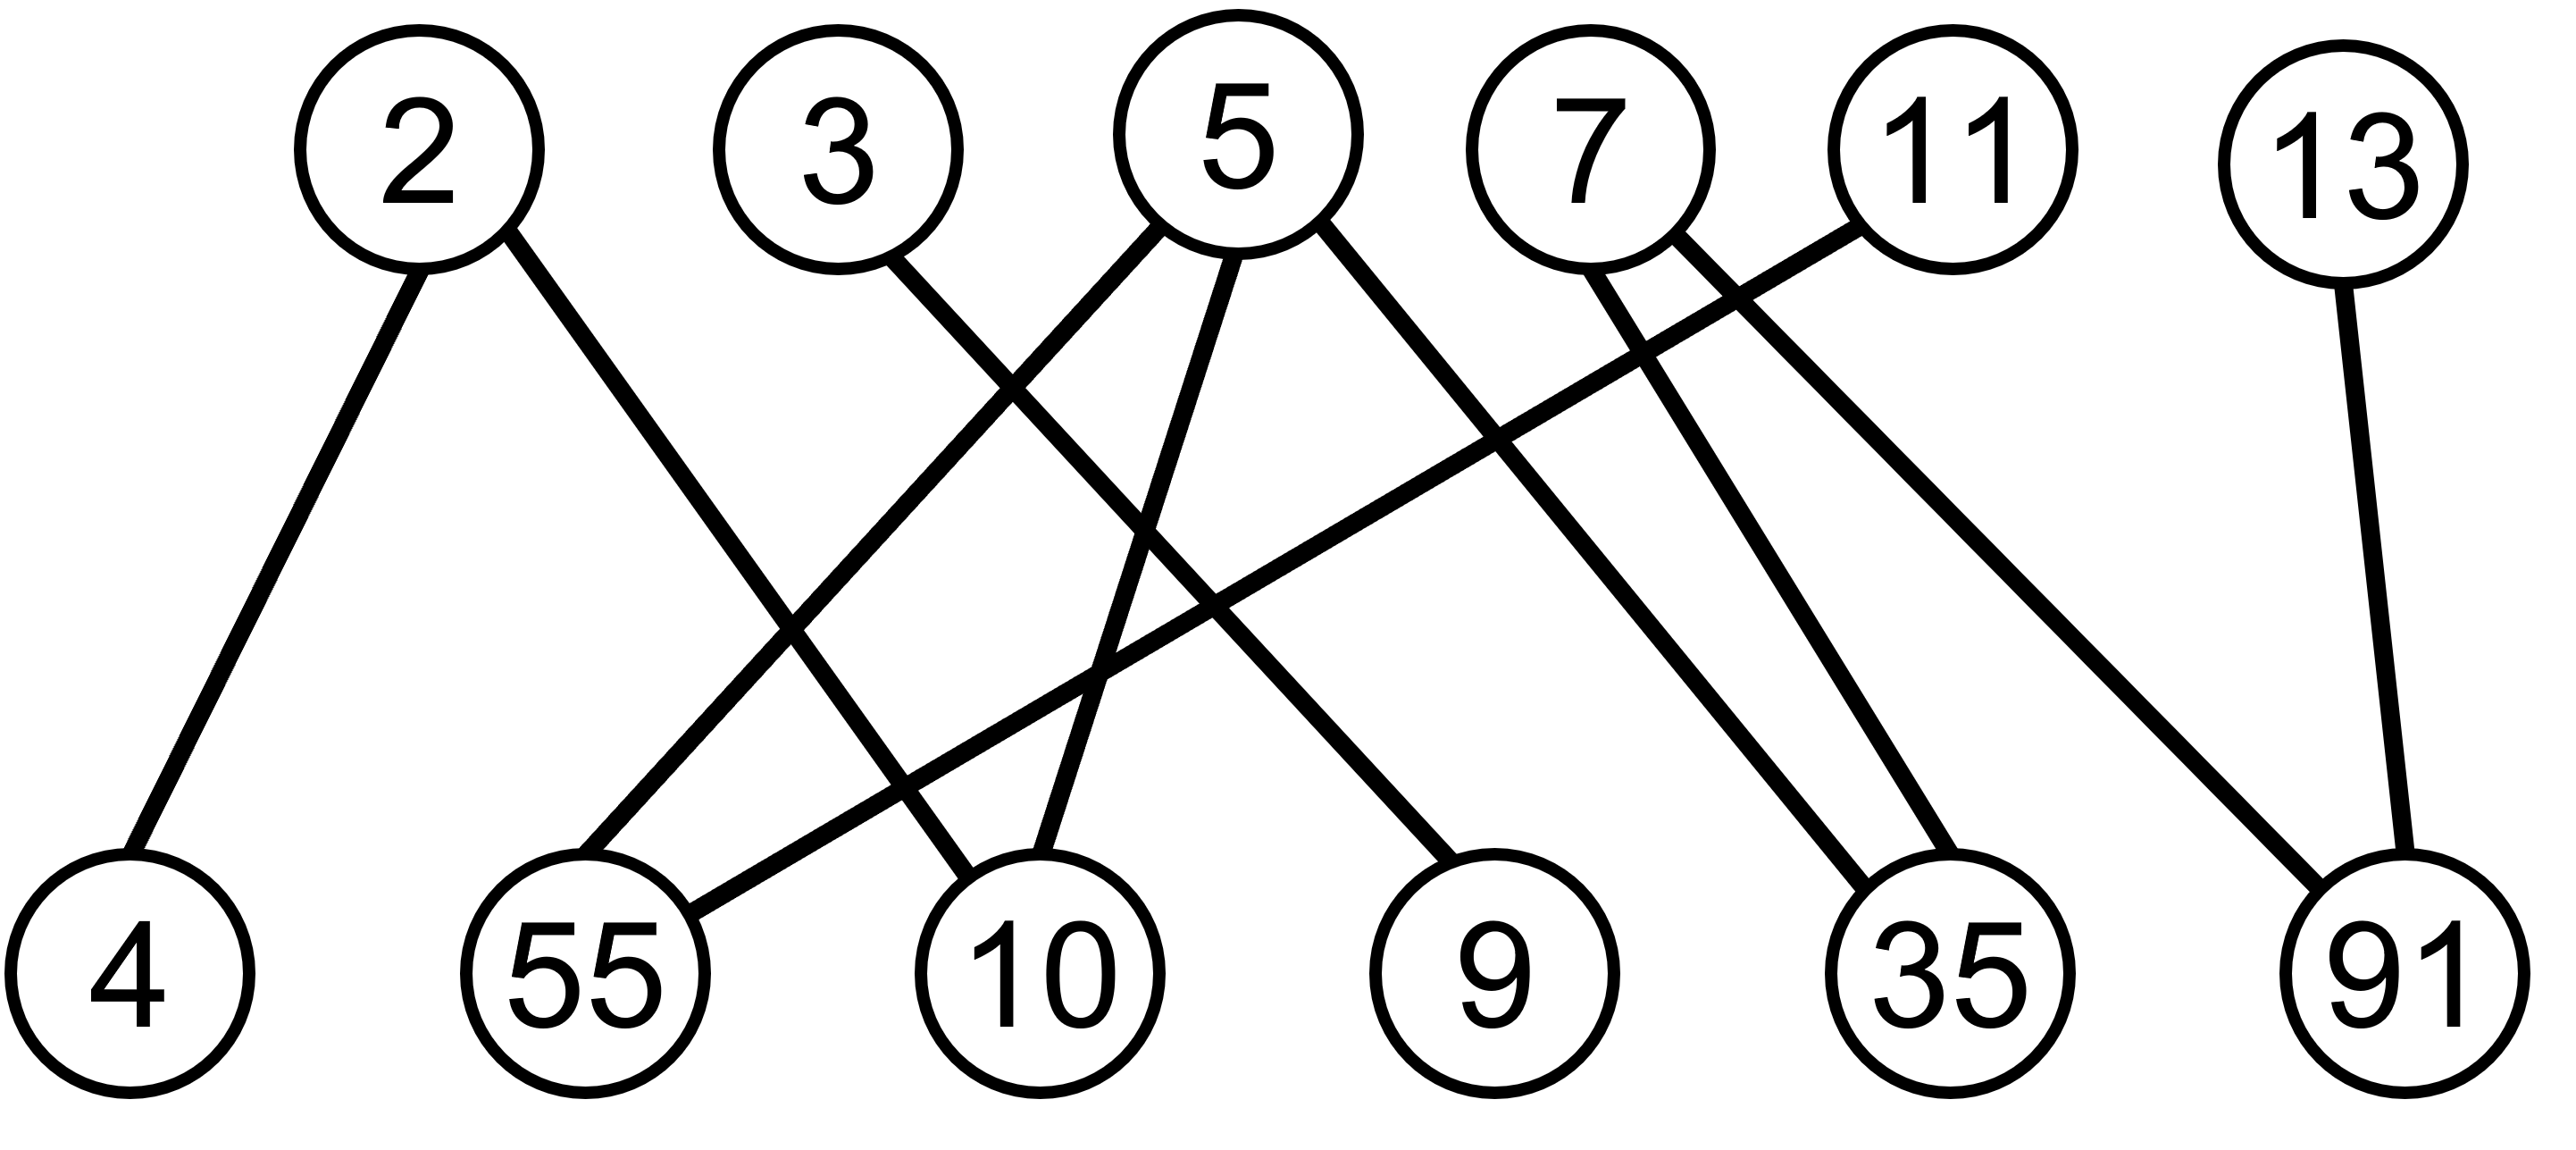
\includegraphics[scale=0.25]{grafos/primos}
\end{center}

Ahora, como todo par de números con MCD distinto a uno comparten por lo menos un primo divisor, podemos hacer un movimiento de ficha yendo del arreglo al primo común a la otra posición del arreglo. Por lo que podemos hacer una BFS en este grafo, aunque habrá que dividir entre dos la respuesta al final.

La lección de este problema es que aprendas a pensar en grafos para resolver problemas, incluso cuando el problema no aparenta ser de grafos.	

\begin{center}
	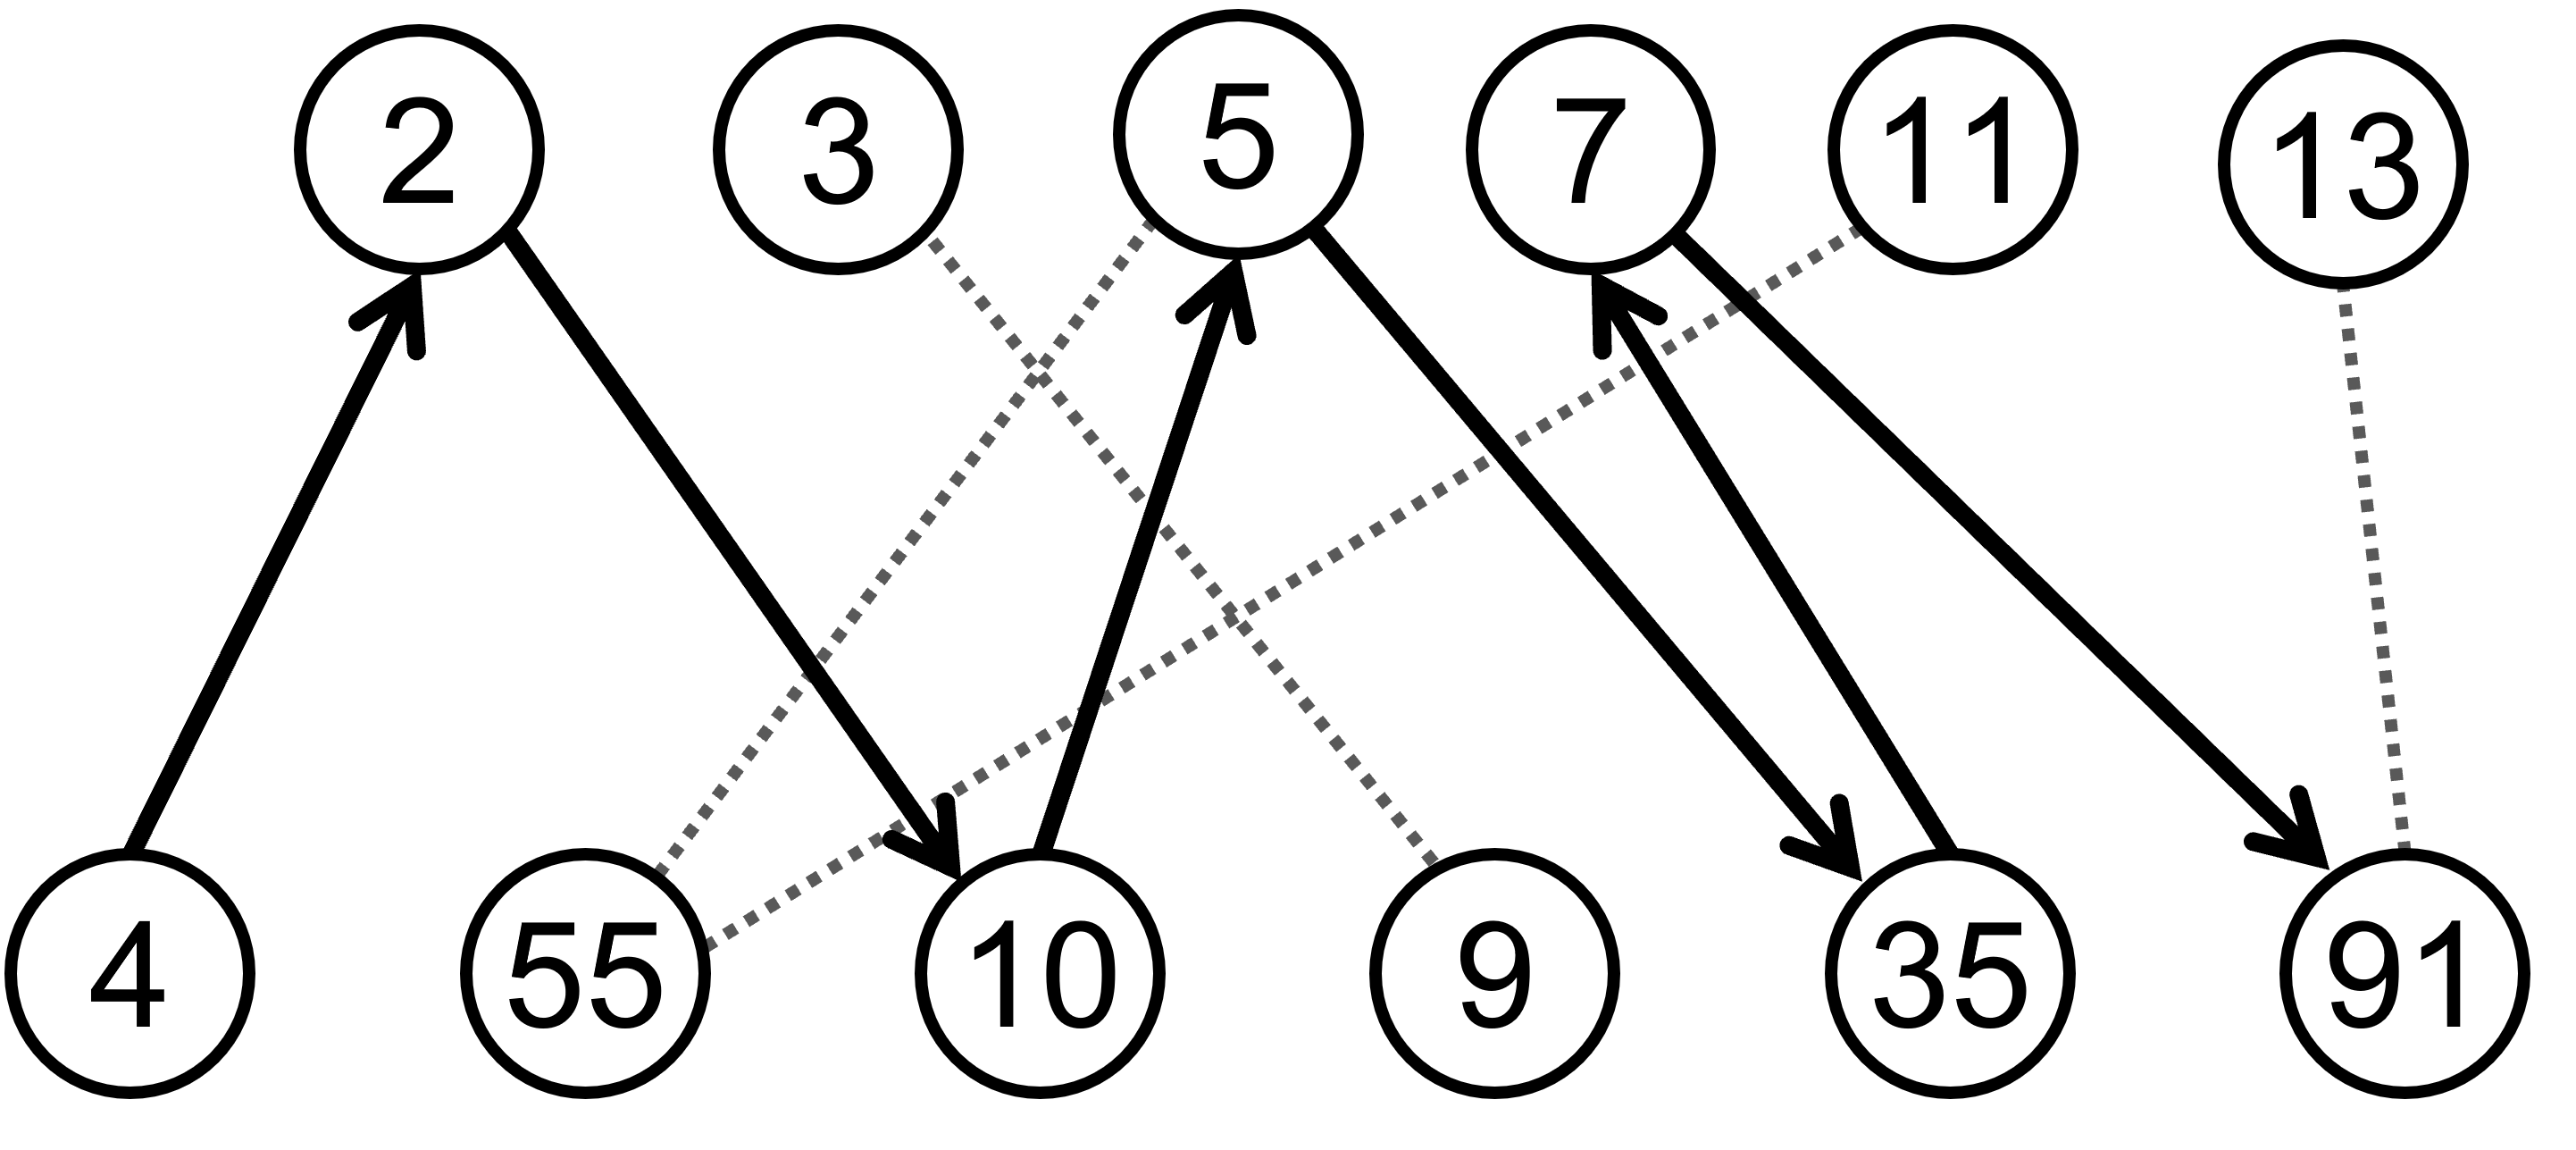
\includegraphics[scale=0.25]{grafos/primos2}
\end{center}